\SourceLeaf{330}\Needspace{28\baselineskip}

\begin{center}
[5.]

[\emph{Handbuch}, S.\ 269 bis 271.]
\end{center}

\begin{center}Zusatz zu p.\ 150 und 201 [des Handbuchs].\end{center}

In Fig.\ I sind die vier gegebenen Punkte und die zwischen ihnen gebildeten Verbindungslinien und Winkel mit ihren Bezeichnungen vorgestellt. Fig.\ II. entsteht, indem man die Winkel $\mathfrak{A}$, $\mathfrak{B}$, $\mathfrak{C}$ beibehält, aber anstatt der Radien $\alpha$, $\beta$, $\gamma$ die reciproken $\dfrac{\alpha\beta\gamma}{\alpha}$, $\dfrac{\alpha\beta\gamma}{\beta}$, $\dfrac{\alpha\beta\gamma}{\gamma}$ annimmt. Die übrigen Bezeichnungen erklären sich von selbst.

\begin{center}
\begin{minipage}[b]{5.5cm}\centering\resizebox{5.2cm}{!}{%
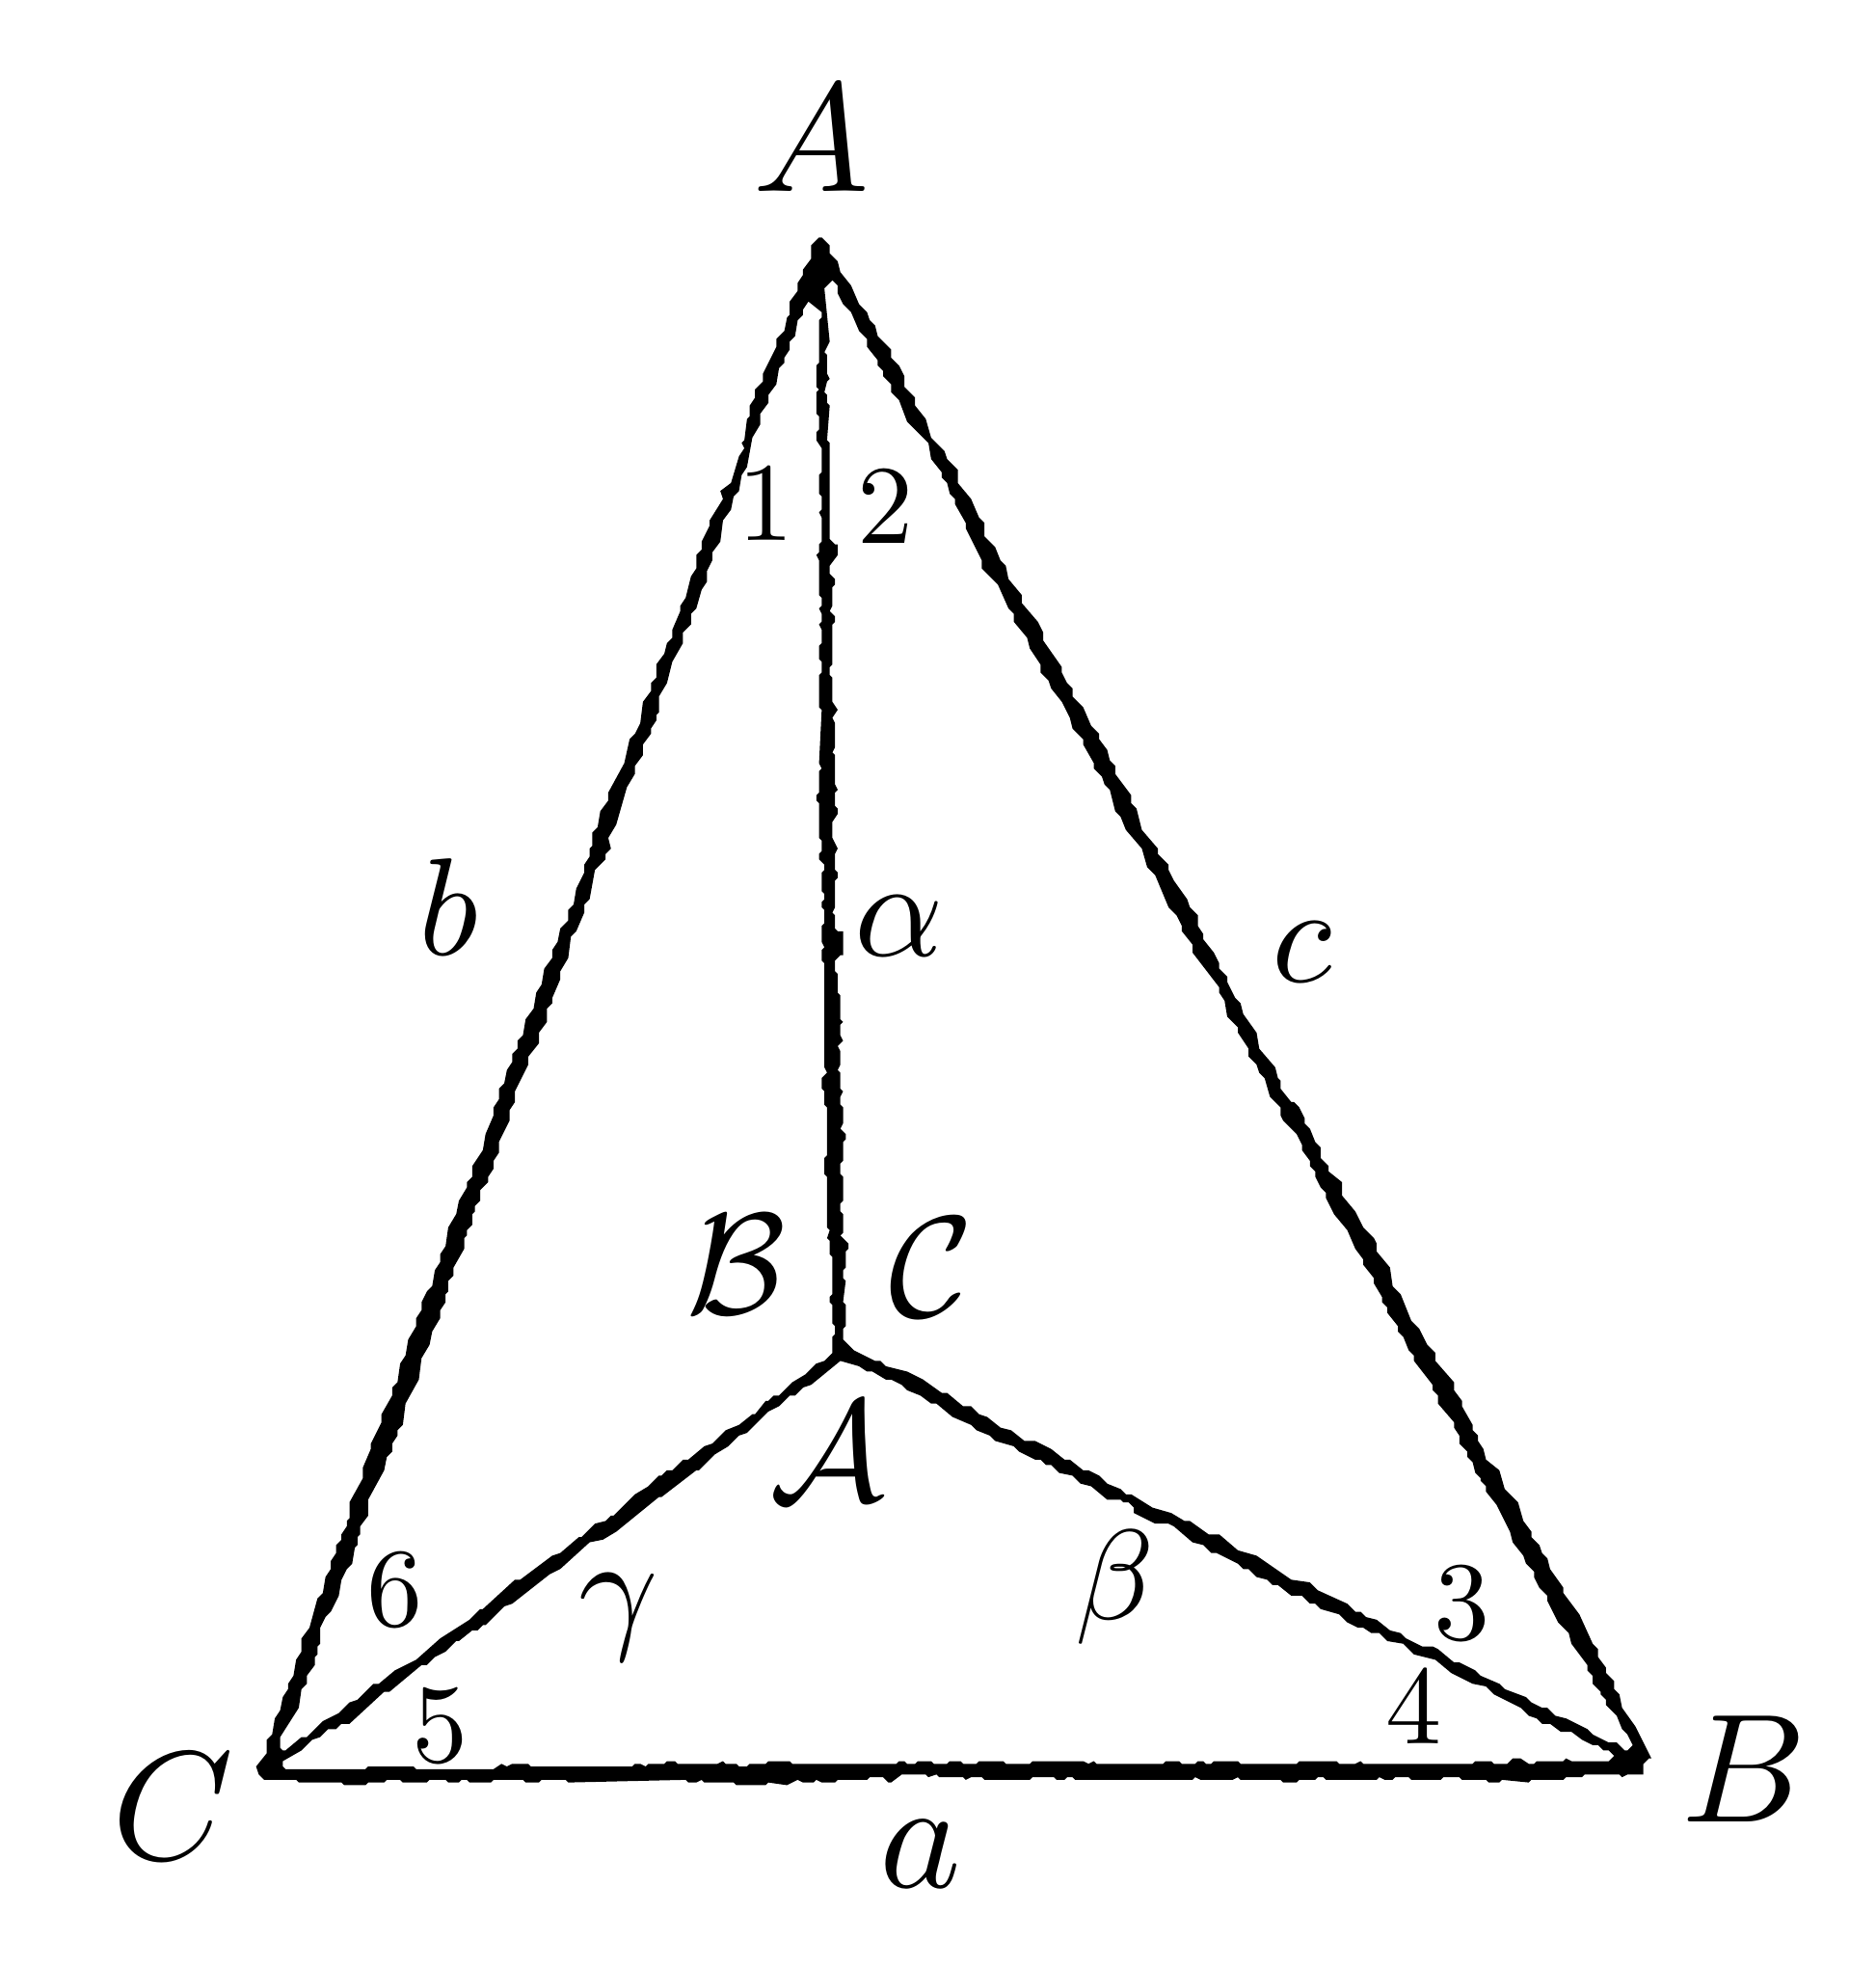
\begin{tikzpicture}[x=1pt,y=-1pt]
\path[use as bounding box] (0,0) rectangle (683,717);
\path[fill=black,draw=none,even odd rule]
(297,79) -- (294,82) -- (294,87) -- (291,91) -- (291,93) -- (289,96) -- (289,99) -- (286,103) -- (286,108) -- (285,109) -- (284,114) -- (281,117) -- (281,120) -- (276,130) -- (276,133) -- (273,136) -- (273,139) -- (271,142) -- (271,146) -- (270,147) -- (269,155) -- (268,156) -- (269,158) -- (267,161) -- (264,171) -- (260,174) -- (261,177) -- (256,185) -- (256,187) -- (253,193) -- (253,196) -- (251,198) -- (251,203) -- (249,206) -- (247,214) -- (245,217) -- (245,219) -- (242,226) -- (242,229) -- (240,231) -- (239,235) -- (236,239) -- (236,244) -- (234,246) -- (234,249) -- (231,253) -- (230,261) -- (228,265) -- (226,267) -- (224,276) -- (218,287) -- (218,290) -- (215,294) -- (214,300) -- (212,302) -- (212,307) -- (211,308) -- (211,311) -- (209,314) -- (209,317) -- (206,323) -- (205,329) -- (203,331) -- (203,335) -- (200,338) -- (199,343) -- (197,346) -- (197,349) -- (194,353) -- (193,359) -- (191,362) -- (190,368) -- (187,372) -- (186,378) -- (184,380) -- (184,383) -- (182,385) -- (182,388) -- (180,391) -- (179,396) -- (177,398) -- (177,402) -- (175,405) -- (175,408) -- (172,415) -- (171,421) -- (167,427) -- (167,431) -- (165,433) -- (165,435) -- (162,440) -- (161,445) -- (158,450) -- (157,457) -- (155,460) -- (155,463) -- (153,466) -- (152,472) -- (150,474) -- (148,478) -- (148,481) -- (146,484) -- (146,487) -- (143,492) -- (142,498) -- (140,501) -- (139,508) -- (137,510) -- (137,513) -- (133,520) -- (133,523) -- (129,531) -- (129,533) -- (126,540) -- (126,544) -- (121,553) -- (121,559) -- (120,560) -- (120,562) -- (118,565) -- (118,567) -- (116,569) -- (116,572) -- (114,575) -- (114,578) -- (112,581) -- (111,587) -- (109,589) -- (106,600) -- (103,604) -- (103,609) -- (101,612) -- (100,618) -- (98,621) -- (98,623) -- (96,626) -- (95,631) -- (93,634) -- (92,640) -- (90,642) -- (90,647) -- (86,652) -- (87,655) -- (89,657) -- (101,657) -- (102,658) -- (118,658) -- (119,659) -- (127,659) -- (128,658) -- (134,658) -- (135,657) -- (140,657) -- (141,658) -- (150,658) -- (151,657) -- (157,657) -- (158,658) -- (162,658) -- (163,657) -- (165,657) -- (166,658) -- (174,658) -- (175,657) -- (186,657) -- (187,658) -- (192,658) -- (193,657) -- (202,657) -- (203,658) -- (247,657) -- (248,658) -- (251,658) -- (253,657) -- (254,658) -- (265,658) -- (266,659) -- (277,659) -- (278,658) -- (285,659) -- (289,657) -- (291,658) -- (295,658) -- (296,657) -- (298,658) -- (303,658) -- (304,657) -- (315,657) -- (316,656) -- (321,656) -- (323,658) -- (324,658) -- (328,655) -- (337,655) -- (338,656) -- (341,655) -- (342,656) -- (351,656) -- (352,657) -- (354,656) -- (358,656) -- (359,657) -- (376,657) -- (377,656) -- (385,656) -- (386,657) -- (389,657) -- (390,656) -- (392,656) -- (393,657) -- (437,657) -- (438,656) -- (440,657) -- (452,657) -- (454,656) -- (455,657) -- (470,657) -- (471,658) -- (476,658) -- (477,657) -- (483,657) -- (484,656) -- (486,656) -- (487,657) -- (506,657) -- (507,656) -- (509,657) -- (512,657) -- (513,656) -- (518,656) -- (519,657) -- (530,657) -- (531,656) -- (537,656) -- (538,657) -- (547,657) -- (548,658) -- (552,658) -- (553,657) -- (563,658) -- (564,657) -- (576,657) -- (577,656) -- (583,656) -- (584,655) -- (597,655) -- (598,656) -- (600,655) -- (606,655) -- (606,651) -- (608,649) -- (609,649) -- (603,637) -- (598,630) -- (597,625) -- (595,623) -- (595,620) -- (592,617) -- (592,615) -- (589,611) -- (589,608) -- (587,606) -- (582,595) -- (576,587) -- (576,585) -- (571,578) -- (570,574) -- (568,572) -- (567,569) -- (564,566) -- (564,564) -- (561,560) -- (559,553) -- (554,548) -- (552,541) -- (547,537) -- (546,533) -- (544,530) -- (544,528) -- (542,526) -- (542,524) -- (538,517) -- (538,515) -- (535,511) -- (535,508) -- (528,500) -- (528,497) -- (525,494) -- (522,488) -- (519,485) -- (515,475) -- (512,472) -- (511,465) -- (506,459) -- (506,456) -- (505,454) -- (501,450) -- (498,444) -- (493,438) -- (493,433) -- (488,429) -- (488,427) -- (485,424) -- (485,420) -- (483,418) -- (481,413) -- (479,411) -- (479,409) -- (477,405) -- (475,403) -- (474,403) -- (470,398) -- (470,395) -- (469,394) -- (468,390) -- (462,383) -- (461,377) -- (456,370) -- (455,366) -- (453,364) -- (450,358) -- (450,356) -- (447,353) -- (447,351) -- (445,347) -- (441,342) -- (441,340) -- (439,337) -- (439,333) -- (436,330) -- (435,327) -- (430,320) -- (428,316) -- (428,314) -- (424,310) -- (424,308) -- (418,301) -- (416,293) -- (414,291) -- (414,288) -- (408,280) -- (408,277) -- (406,275) -- (405,271) -- (402,267) -- (402,265) -- (399,262) -- (396,255) -- (392,251) -- (392,248) -- (390,246) -- (388,242) -- (388,240) -- (381,230) -- (381,227) -- (379,223) -- (373,216) -- (373,213) -- (368,207) -- (367,202) -- (365,200) -- (363,195) -- (359,191) -- (359,186) -- (357,184) -- (354,177) -- (349,171) -- (349,166) -- (345,162) -- (344,159) -- (339,154) -- (337,147) -- (333,142) -- (333,139) -- (329,135) -- (329,131) -- (327,127) -- (324,124) -- (324,121) -- (319,116) -- (318,112) -- (316,110) -- (315,107) -- (312,104) -- (309,97) -- (305,92) -- (304,88) -- (301,85) -- (301,82) -- (298,79) -- cycle
(96,652) -- (96,650) -- (103,646) -- (107,642) -- (110,641) -- (113,638) -- (116,638) -- (118,636) -- (121,636) -- (134,624) -- (136,624) -- (148,614) -- (150,614) -- (153,611) -- (157,609) -- (161,605) -- (162,605) -- (167,601) -- (169,601) -- (171,599) -- (172,599) -- (179,592) -- (182,591) -- (196,580) -- (200,578) -- (211,568) -- (216,567) -- (221,564) -- (237,551) -- (238,551) -- (251,541) -- (252,541) -- (258,535) -- (263,532) -- (267,528) -- (270,527) -- (278,519) -- (282,517) -- (286,513) -- (288,513) -- (291,510) -- (294,509) -- (305,500) -- (312,502) -- (315,504) -- (317,504) -- (322,507) -- (324,507) -- (328,509) -- (330,511) -- (335,513) -- (339,516) -- (341,516) -- (347,521) -- (354,524) -- (356,526) -- (361,528) -- (363,530) -- (370,532) -- (372,534) -- (378,537) -- (380,537) -- (382,539) -- (384,539) -- (387,542) -- (392,543) -- (395,546) -- (399,547) -- (405,552) -- (410,552) -- (411,553) -- (413,553) -- (415,555) -- (415,557) -- (423,561) -- (428,561) -- (430,562) -- (437,568) -- (441,569) -- (444,572) -- (446,572) -- (454,576) -- (456,578) -- (458,578) -- (461,581) -- (465,582) -- (467,584) -- (469,584) -- (474,588) -- (478,588) -- (481,591) -- (483,591) -- (485,593) -- (492,595) -- (495,598) -- (499,600) -- (501,600) -- (504,602) -- (507,602) -- (510,605) -- (516,606) -- (520,610) -- (528,612) -- (534,617) -- (542,621) -- (547,622) -- (550,625) -- (560,630) -- (563,633) -- (566,634) -- (568,636) -- (571,636) -- (575,639) -- (579,639) -- (583,642) -- (587,644) -- (589,644) -- (591,646) -- (593,646) -- (595,648) -- (593,650) -- (579,650) -- (577,649) -- (576,650) -- (566,650) -- (565,651) -- (563,651) -- (560,649) -- (557,649) -- (555,651) -- (550,651) -- (549,650) -- (543,650) -- (542,651) -- (501,651) -- (500,650) -- (498,651) -- (492,651) -- (491,650) -- (477,650) -- (476,651) -- (455,651) -- (454,650) -- (445,650) -- (444,651) -- (442,651) -- (441,650) -- (439,650) -- (438,651) -- (433,651) -- (432,650) -- (427,650) -- (426,651) -- (401,651) -- (400,650) -- (398,651) -- (396,650) -- (377,650) -- (376,651) -- (367,651) -- (366,650) -- (357,650) -- (356,651) -- (351,651) -- (350,650) -- (346,650) -- (345,651) -- (340,651) -- (339,650) -- (334,650) -- (333,651) -- (330,651) -- (329,650) -- (327,650) -- (326,651) -- (287,651) -- (286,650) -- (278,650) -- (277,651) -- (271,651) -- (270,652) -- (267,652) -- (266,651) -- (262,651) -- (261,650) -- (259,651) -- (244,651) -- (243,650) -- (240,650) -- (239,651) -- (233,651) -- (232,652) -- (230,651) -- (228,651) -- (227,652) -- (189,652) -- (188,651) -- (182,651) -- (180,652) -- (178,651) -- (175,653) -- (146,653) -- (145,652) -- (128,652) -- (127,653) -- (97,653) -- cycle
(293,103) -- (298,107) -- (298,109) -- (297,110) -- (297,126) -- (296,127) -- (296,135) -- (297,136) -- (296,137) -- (296,145) -- (297,146) -- (297,151) -- (296,152) -- (296,155) -- (298,158) -- (298,167) -- (297,168) -- (297,175) -- (298,176) -- (298,181) -- (297,182) -- (298,184) -- (298,193) -- (297,194) -- (297,197) -- (296,198) -- (297,200) -- (297,213) -- (298,214) -- (298,217) -- (297,218) -- (298,220) -- (298,223) -- (297,224) -- (298,226) -- (298,231) -- (297,232) -- (297,237) -- (298,238) -- (298,242) -- (297,243) -- (297,255) -- (298,256) -- (297,276) -- (298,278) -- (297,279) -- (297,287) -- (296,288) -- (296,290) -- (297,291) -- (297,304) -- (298,305) -- (298,309) -- (297,310) -- (297,312) -- (299,314) -- (299,316) -- (298,317) -- (298,324) -- (299,325) -- (299,327) -- (298,328) -- (298,330) -- (299,331) -- (299,336) -- (298,337) -- (298,343) -- (299,345) -- (298,346) -- (298,350) -- (299,351) -- (299,390) -- (300,392) -- (298,394) -- (298,398) -- (299,399) -- (299,404) -- (300,405) -- (300,423) -- (299,424) -- (299,430) -- (300,431) -- (300,450) -- (301,451) -- (300,454) -- (301,455) -- (301,460) -- (302,461) -- (302,475) -- (301,476) -- (301,478) -- (302,479) -- (302,486) -- (303,487) -- (303,490) -- (302,491) -- (302,497) -- (299,500) -- (296,501) -- (292,505) -- (287,508) -- (282,513) -- (280,513) -- (278,515) -- (277,515) -- (273,520) -- (272,520) -- (267,524) -- (262,526) -- (257,531) -- (254,532) -- (248,537) -- (246,537) -- (242,541) -- (240,541) -- (238,543) -- (237,543) -- (233,547) -- (228,550) -- (220,558) -- (219,558) -- (217,560) -- (213,561) -- (208,566) -- (207,566) -- (200,572) -- (197,573) -- (185,582) -- (183,582) -- (171,593) -- (170,593) -- (166,597) -- (155,604) -- (146,612) -- (138,616) -- (132,621) -- (130,621) -- (124,627) -- (121,628) -- (117,632) -- (111,635) -- (105,641) -- (103,641) -- (97,646) -- (96,646) -- (95,645) -- (95,641) -- (102,630) -- (103,623) -- (105,621) -- (105,618) -- (108,614) -- (108,611) -- (109,610) -- (109,607) -- (110,606) -- (110,600) -- (112,596) -- (114,594) -- (117,588) -- (118,582) -- (120,578) -- (122,576) -- (123,570) -- (124,569) -- (124,566) -- (125,565) -- (125,562) -- (128,558) -- (128,552) -- (134,541) -- (135,536) -- (137,534) -- (137,531) -- (139,528) -- (139,526) -- (141,524) -- (142,516) -- (147,507) -- (148,499) -- (151,494) -- (152,489) -- (155,484) -- (155,481) -- (157,478) -- (157,475) -- (158,474) -- (158,470) -- (160,468) -- (160,465) -- (164,458) -- (164,454) -- (165,453) -- (165,451) -- (167,449) -- (167,445) -- (168,444) -- (168,442) -- (170,440) -- (170,436) -- (173,433) -- (173,431) -- (175,428) -- (175,425) -- (177,422) -- (177,418) -- (181,410) -- (181,406) -- (183,403) -- (183,399) -- (188,389) -- (188,386) -- (192,381) -- (192,377) -- (195,373) -- (195,368) -- (197,366) -- (197,364) -- (200,357) -- (200,354) -- (203,349) -- (204,341) -- (206,339) -- (209,332) -- (209,329) -- (211,327) -- (213,316) -- (217,312) -- (217,310) -- (219,308) -- (218,304) -- (221,299) -- (225,285) -- (228,280) -- (228,277) -- (231,273) -- (231,269) -- (234,265) -- (234,263) -- (236,260) -- (236,258) -- (237,257) -- (237,251) -- (240,246) -- (242,238) -- (246,231) -- (246,227) -- (249,224) -- (249,220) -- (251,218) -- (253,211) -- (255,208) -- (255,204) -- (257,200) -- (257,197) -- (260,193) -- (261,185) -- (264,181) -- (265,176) -- (267,174) -- (268,168) -- (270,165) -- (272,154) -- (275,149) -- (275,145) -- (278,141) -- (278,138) -- (281,134) -- (282,128) -- (284,126) -- (284,124) -- (286,121) -- (286,118) -- (288,116) -- (289,110) -- (291,108) -- (291,106) -- cycle
(302,95) -- (304,97) -- (304,100) -- (306,104) -- (309,107) -- (312,114) -- (315,117) -- (315,120) -- (319,125) -- (319,127) -- (321,129) -- (321,131) -- (324,134) -- (324,137) -- (327,140) -- (330,148) -- (338,156) -- (339,162) -- (343,167) -- (343,169) -- (345,171) -- (346,175) -- (348,177) -- (348,179) -- (352,186) -- (352,188) -- (358,200) -- (358,203) -- (364,209) -- (368,218) -- (370,220) -- (370,223) -- (375,229) -- (376,233) -- (380,239) -- (380,242) -- (383,245) -- (384,248) -- (388,253) -- (391,259) -- (392,263) -- (396,267) -- (396,269) -- (400,276) -- (400,278) -- (403,281) -- (404,284) -- (406,286) -- (408,294) -- (410,296) -- (412,301) -- (418,308) -- (420,315) -- (423,318) -- (428,330) -- (431,333) -- (433,337) -- (433,339) -- (437,344) -- (437,347) -- (447,360) -- (447,362) -- (449,365) -- (450,371) -- (454,375) -- (454,377) -- (458,383) -- (458,386) -- (461,389) -- (462,392) -- (464,394) -- (466,401) -- (470,405) -- (470,408) -- (471,410) -- (476,415) -- (478,419) -- (478,421) -- (481,425) -- (481,427) -- (483,429) -- (483,431) -- (485,435) -- (487,437) -- (487,439) -- (490,445) -- (495,451) -- (498,458) -- (501,462) -- (501,464) -- (505,469) -- (505,471) -- (508,476) -- (508,478) -- (510,480) -- (510,482) -- (514,487) -- (514,489) -- (516,491) -- (518,496) -- (520,498) -- (520,500) -- (527,509) -- (527,511) -- (529,513) -- (529,516) -- (535,523) -- (535,525) -- (537,528) -- (537,531) -- (540,534) -- (540,536) -- (542,538) -- (543,542) -- (545,544) -- (545,545) -- (547,547) -- (547,549) -- (551,554) -- (556,564) -- (557,568) -- (561,573) -- (562,576) -- (565,579) -- (565,581) -- (567,585) -- (570,588) -- (570,590) -- (574,598) -- (578,602) -- (579,606) -- (585,614) -- (585,616) -- (587,618) -- (587,621) -- (590,624) -- (590,625) -- (592,627) -- (592,629) -- (596,633) -- (598,638) -- (600,640) -- (602,644) -- (600,646) -- (599,646) -- (596,643) -- (593,643) -- (587,640) -- (585,638) -- (577,634) -- (573,633) -- (570,630) -- (568,630) -- (564,628) -- (562,626) -- (554,623) -- (552,621) -- (545,618) -- (543,616) -- (537,613) -- (535,613) -- (529,608) -- (527,607) -- (523,607) -- (517,604) -- (515,602) -- (511,601) -- (506,597) -- (502,596) -- (500,594) -- (498,594) -- (495,591) -- (484,586) -- (481,583) -- (474,582) -- (461,573) -- (454,571) -- (447,565) -- (443,565) -- (436,560) -- (434,560) -- (429,557) -- (422,555) -- (414,550) -- (412,550) -- (410,548) -- (405,546) -- (402,543) -- (398,541) -- (396,541) -- (391,537) -- (389,537) -- (384,533) -- (378,530) -- (374,530) -- (369,526) -- (365,525) -- (360,521) -- (357,520) -- (354,517) -- (351,517) -- (345,512) -- (343,512) -- (336,507) -- (330,504) -- (322,502) -- (320,500) -- (318,500) -- (310,496) -- (306,492) -- (306,488) -- (307,487) -- (307,479) -- (306,478) -- (307,470) -- (306,469) -- (306,466) -- (307,465) -- (307,459) -- (308,458) -- (308,456) -- (305,453) -- (306,452) -- (306,445) -- (305,444) -- (305,441) -- (306,440) -- (306,431) -- (305,430) -- (305,426) -- (306,425) -- (306,418) -- (307,417) -- (307,415) -- (305,413) -- (306,411) -- (306,405) -- (305,404) -- (305,401) -- (306,399) -- (305,398) -- (305,392) -- (304,391) -- (305,389) -- (305,384) -- (304,382) -- (306,380) -- (305,378) -- (305,374) -- (306,373) -- (305,372) -- (305,363) -- (304,362) -- (304,355) -- (303,354) -- (303,350) -- (305,348) -- (306,348) -- (306,339) -- (304,339) -- (303,338) -- (303,333) -- (302,332) -- (303,330) -- (303,320) -- (304,319) -- (304,317) -- (303,316) -- (303,310) -- (304,308) -- (302,304) -- (302,298) -- (304,295) -- (304,293) -- (303,292) -- (303,287) -- (304,286) -- (303,284) -- (303,273) -- (302,272) -- (303,270) -- (303,261) -- (302,259) -- (304,256) -- (302,253) -- (302,244) -- (301,243) -- (301,240) -- (302,239) -- (302,224) -- (303,223) -- (303,221) -- (301,219) -- (302,217) -- (302,210) -- (303,209) -- (303,207) -- (301,205) -- (301,202) -- (304,198) -- (304,194) -- (303,194) -- (301,192) -- (301,156) -- (300,155) -- (301,142) -- (300,141) -- (300,138) -- (299,137) -- (300,133) -- (301,132) -- (300,130) -- (300,123) -- (299,122) -- (301,118) -- (299,98) -- cycle;
\node[inner sep=0pt,font=\fontsize{10}{10}\selectfont] at (294,42) {\scalebox{5.8}{$A$}};
\node[inner sep=0pt,font=\fontsize{10}{10}\selectfont] at (644,653) {\scalebox{5.8}{$B$}};
\node[inner sep=0pt,font=\fontsize{10}{10}\selectfont] at (55,667) {\scalebox{5.8}{$C$}};
\node[inner sep=0pt,font=\fontsize{10}{10}\selectfont] at (335,685) {\scalebox{5.8}{$a$}};
\node[inner sep=0pt,font=\fontsize{10}{10}\selectfont] at (158,330) {\scalebox{5.2}{$b$}};
\node[inner sep=0pt,font=\fontsize{10}{10}\selectfont] at (478,347) {\scalebox{5.2}{$c$}};
\node[inner sep=0pt,font=\fontsize{10}{10}\selectfont] at (327,337) {\scalebox{5.2}{$\alpha$}};
\node[inner sep=0pt,font=\fontsize{10}{10}\selectfont] at (408,585) {\scalebox{4.8}{$\beta$}};
\node[inner sep=0pt,font=\fontsize{10}{10}\selectfont] at (222,596) {\scalebox{5.2}{$\gamma$}};
\node[inner sep=0pt,font=\fontsize{10}{10}\selectfont] at (266,464) {\scalebox{5.4}{$\mathcal{B}$}};
\node[inner sep=0pt,font=\fontsize{10}{10}\selectfont] at (339,465) {\scalebox{5.4}{$\mathcal{C}$}};
\node[inner sep=0pt,font=\fontsize{10}{10}\selectfont] at (300,534) {\scalebox{5.4}{$\mathcal{A}$}};
\node[inner sep=0pt,font=\fontsize{10}{10}\selectfont] at (277,179) {\scalebox{4.2}{$1$}};
\node[inner sep=0pt,font=\fontsize{10}{10}\selectfont] at (322,180) {\scalebox{4.2}{$2$}};
\node[inner sep=0pt,font=\fontsize{10}{10}\selectfont] at (538,591) {\scalebox{4.2}{$3$}};
\node[inner sep=0pt,font=\fontsize{10}{10}\selectfont] at (520,630) {\scalebox{4.2}{$4$}};
\node[inner sep=0pt,font=\fontsize{10}{10}\selectfont] at (155,637) {\scalebox{4.2}{$5$}};
\node[inner sep=0pt,font=\fontsize{10}{10}\selectfont] at (138,586) {\scalebox{4.2}{$6$}};
\end{tikzpicture}%
}
\\Fig.\ I.\end{minipage}\hspace{.3cm}%
\begin{minipage}[b]{6.6cm}\centering\resizebox{6.4cm}{!}{%
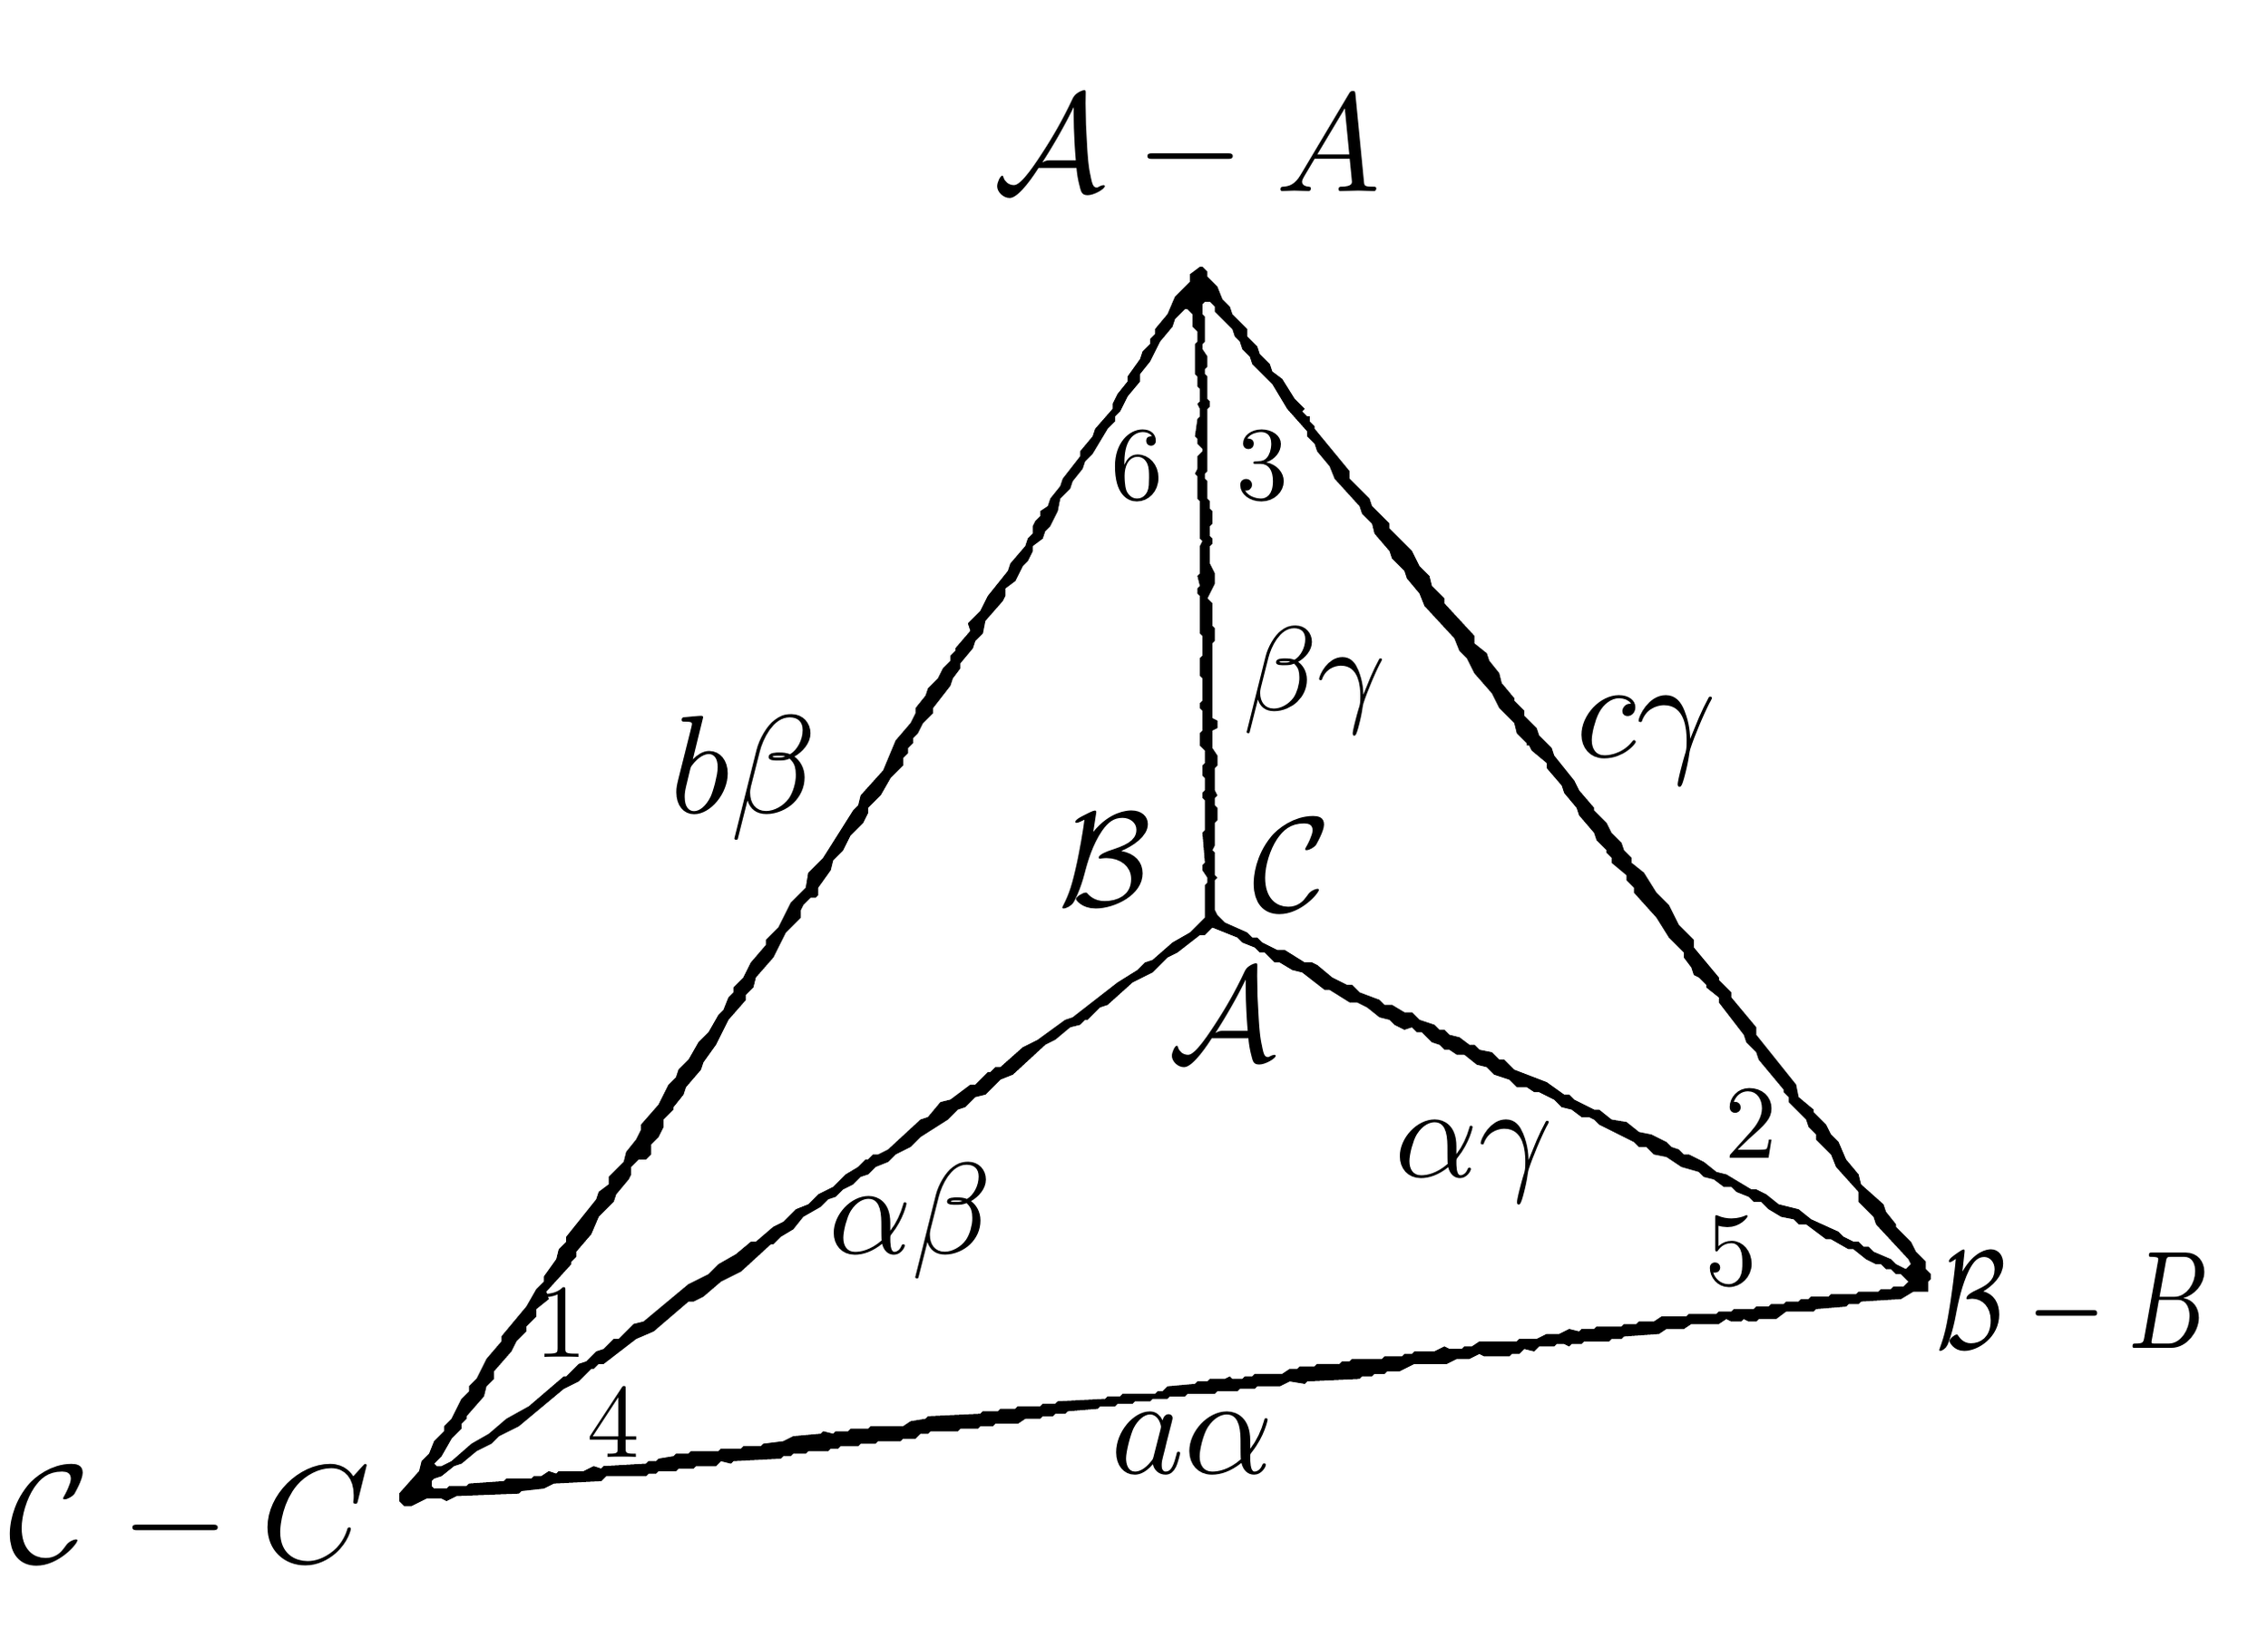
\begin{tikzpicture}[x=1pt,y=-1pt]
\path[use as bounding box] (0,0) rectangle (889,633);
\path[fill=black,draw=none,even odd rule]
(764,501) -- (762,499) -- (762,496) -- (758,492) -- (756,488) -- (750,482) -- (750,481) -- (746,476) -- (745,473) -- (736,465) -- (735,461) -- (730,455) -- (727,448) -- (724,445) -- (722,441) -- (717,436) -- (717,435) -- (711,430) -- (710,425) -- (694,405) -- (694,402) -- (684,390) -- (684,388) -- (679,383) -- (679,382) -- (669,370) -- (669,367) -- (663,361) -- (659,353) -- (654,348) -- (649,340) -- (644,336) -- (644,334) -- (641,331) -- (640,328) -- (636,324) -- (634,320) -- (629,315) -- (629,314) -- (623,307) -- (621,303) -- (613,293) -- (612,290) -- (607,285) -- (606,282) -- (601,277) -- (601,275) -- (597,271) -- (597,270) -- (592,264) -- (591,260) -- (587,255) -- (586,252) -- (581,248) -- (581,245) -- (569,232) -- (569,230) -- (564,225) -- (563,221) -- (559,217) -- (556,211) -- (547,202) -- (547,200) -- (540,193) -- (539,190) -- (531,182) -- (531,179) -- (517,162) -- (517,161) -- (515,159) -- (515,157) -- (514,157) -- (512,155) -- (513,154) -- (509,150) -- (504,142) -- (500,139) -- (499,136) -- (495,132) -- (494,129) -- (490,125) -- (490,122) -- (484,116) -- (483,113) -- (480,110) -- (478,105) -- (474,101) -- (474,99) -- (472,97) -- (471,97) -- (467,100) -- (467,103) -- (461,109) -- (458,116) -- (453,122) -- (453,124) -- (451,126) -- (451,128) -- (448,131) -- (447,134) -- (442,141) -- (442,143) -- (438,148) -- (436,152) -- (436,154) -- (429,162) -- (428,165) -- (423,171) -- (423,173) -- (416,182) -- (415,185) -- (411,190) -- (410,193) -- (407,195) -- (407,197) -- (405,199) -- (404,201) -- (404,204) -- (402,206) -- (401,209) -- (395,216) -- (394,219) -- (386,229) -- (383,235) -- (378,240) -- (379,243) -- (373,250) -- (373,251) -- (371,253) -- (371,255) -- (368,258) -- (366,262) -- (362,266) -- (361,269) -- (357,274) -- (357,276) -- (355,280) -- (349,287) -- (344,299) -- (335,309) -- (334,313) -- (332,315) -- (320,334) -- (314,340) -- (313,346) -- (307,352) -- (302,362) -- (297,367) -- (297,369) -- (291,376) -- (288,382) -- (284,386) -- (284,388) -- (282,390) -- (280,395) -- (278,397) -- (274,404) -- (270,408) -- (266,415) -- (262,419) -- (261,422) -- (258,425) -- (254,433) -- (247,441) -- (247,443) -- (245,447) -- (241,452) -- (240,456) -- (234,462) -- (234,465) -- (230,468) -- (229,471) -- (217,486) -- (217,488) -- (214,491) -- (213,495) -- (208,502) -- (208,504) -- (205,507) -- (201,514) -- (191,526) -- (191,528) -- (185,535) -- (181,543) -- (178,546) -- (178,548) -- (175,551) -- (171,559) -- (168,562) -- (168,564) -- (164,568) -- (162,573) -- (159,576) -- (158,580) -- (150,589) -- (150,592) -- (152,594) -- (155,594) -- (161,591) -- (167,591) -- (169,592) -- (173,590) -- (198,589) -- (199,588) -- (208,587) -- (212,585) -- (231,584) -- (233,582) -- (249,582) -- (250,581) -- (253,581) -- (254,580) -- (261,580) -- (262,579) -- (268,579) -- (269,578) -- (277,578) -- (279,576) -- (283,577) -- (284,576) -- (303,575) -- (304,574) -- (307,574) -- (308,573) -- (313,573) -- (314,572) -- (322,572) -- (323,571) -- (326,571) -- (327,570) -- (334,570) -- (335,569) -- (341,569) -- (342,568) -- (351,568) -- (352,567) -- (357,567) -- (359,565) -- (362,565) -- (363,564) -- (374,564) -- (375,563) -- (382,563) -- (383,562) -- (388,562) -- (389,561) -- (398,561) -- (401,559) -- (407,559) -- (408,558) -- (412,558) -- (413,557) -- (417,557) -- (418,556) -- (430,555) -- (431,554) -- (437,554) -- (438,553) -- (444,553) -- (445,552) -- (451,552) -- (452,551) -- (458,551) -- (459,550) -- (465,550) -- (466,549) -- (477,549) -- (478,548) -- (486,548) -- (487,547) -- (493,547) -- (494,546) -- (503,546) -- (507,544) -- (513,545) -- (514,544) -- (535,543) -- (536,542) -- (540,542) -- (541,541) -- (545,541) -- (546,540) -- (551,540) -- (557,537) -- (570,537) -- (574,535) -- (579,535) -- (583,533) -- (585,534) -- (595,534) -- (596,533) -- (599,533) -- (601,531) -- (605,532) -- (607,530) -- (613,530) -- (614,529) -- (617,529) -- (619,530) -- (620,529) -- (624,529) -- (625,528) -- (635,528) -- (636,527) -- (640,527) -- (641,526) -- (655,525) -- (658,523) -- (665,523) -- (668,521) -- (679,521) -- (682,519) -- (684,520) -- (688,520) -- (689,519) -- (691,520) -- (694,520) -- (695,519) -- (702,519) -- (706,516) -- (717,516) -- (718,515) -- (730,514) -- (731,513) -- (735,513) -- (736,512) -- (752,511) -- (757,508) -- (763,508) -- (763,504) -- (764,503) -- cycle
(755,504) -- (753,506) -- (749,506) -- (748,507) -- (744,507) -- (743,508) -- (735,508) -- (734,509) -- (724,509) -- (723,510) -- (716,510) -- (715,511) -- (712,511) -- (711,512) -- (706,512) -- (705,513) -- (700,513) -- (699,514) -- (694,514) -- (693,515) -- (685,515) -- (684,516) -- (679,516) -- (678,517) -- (667,517) -- (666,518) -- (656,518) -- (653,520) -- (647,520) -- (646,521) -- (641,521) -- (640,522) -- (630,522) -- (629,523) -- (624,523) -- (623,524) -- (619,523) -- (615,525) -- (610,525) -- (606,527) -- (599,527) -- (598,528) -- (583,528) -- (580,530) -- (577,530) -- (576,531) -- (571,531) -- (569,530) -- (565,532) -- (557,532) -- (556,533) -- (553,533) -- (552,534) -- (545,534) -- (544,535) -- (532,535) -- (531,536) -- (528,536) -- (527,537) -- (518,537) -- (517,538) -- (511,538) -- (510,539) -- (507,539) -- (504,541) -- (493,541) -- (492,542) -- (489,542) -- (488,543) -- (484,543) -- (483,542) -- (481,543) -- (475,543) -- (474,544) -- (470,544) -- (469,545) -- (458,546) -- (456,548) -- (454,548) -- (453,549) -- (440,549) -- (439,550) -- (434,550) -- (433,551) -- (414,552) -- (413,553) -- (408,553) -- (407,554) -- (398,554) -- (397,555) -- (391,555) -- (390,556) -- (384,556) -- (383,557) -- (362,558) -- (361,559) -- (355,560) -- (352,562) -- (339,562) -- (338,563) -- (331,563) -- (330,564) -- (325,564) -- (324,565) -- (320,564) -- (319,565) -- (308,566) -- (304,568) -- (296,569) -- (295,570) -- (288,570) -- (287,571) -- (279,571) -- (278,572) -- (267,572) -- (266,573) -- (261,573) -- (260,574) -- (254,575) -- (253,576) -- (250,576) -- (249,577) -- (232,578) -- (231,579) -- (228,578) -- (224,580) -- (214,580) -- (213,581) -- (210,580) -- (207,582) -- (204,582) -- (203,583) -- (193,583) -- (192,584) -- (178,585) -- (177,586) -- (170,586) -- (169,587) -- (164,587) -- (163,586) -- (163,584) -- (164,583) -- (167,582) -- (172,578) -- (175,577) -- (181,572) -- (187,569) -- (190,566) -- (198,562) -- (216,547) -- (222,544) -- (227,539) -- (228,539) -- (230,537) -- (232,537) -- (245,527) -- (252,524) -- (266,512) -- (268,512) -- (272,510) -- (279,504) -- (287,500) -- (299,489) -- (300,489) -- (303,486) -- (308,483) -- (312,478) -- (319,474) -- (322,471) -- (325,470) -- (328,467) -- (332,465) -- (335,462) -- (338,461) -- (341,458) -- (346,456) -- (349,453) -- (355,450) -- (359,446) -- (370,439) -- (374,435) -- (377,434) -- (381,430) -- (385,429) -- (391,423) -- (396,421) -- (409,409) -- (413,407) -- (419,402) -- (423,401) -- (425,399) -- (426,399) -- (431,394) -- (434,393) -- (444,384) -- (452,380) -- (458,374) -- (462,372) -- (471,365) -- (473,365) -- (476,362) -- (486,366) -- (488,368) -- (493,370) -- (495,372) -- (497,372) -- (501,376) -- (503,376) -- (508,379) -- (512,380) -- (521,387) -- (523,387) -- (531,392) -- (534,392) -- (538,394) -- (543,398) -- (547,399) -- (549,401) -- (553,403) -- (556,402) -- (558,404) -- (560,404) -- (564,408) -- (567,409) -- (569,411) -- (571,411) -- (574,413) -- (577,413) -- (582,417) -- (586,418) -- (589,421) -- (595,423) -- (598,426) -- (602,426) -- (605,428) -- (607,428) -- (613,431) -- (616,434) -- (620,435) -- (624,438) -- (627,438) -- (629,439) -- (631,441) -- (645,448) -- (647,450) -- (650,450) -- (653,453) -- (658,454) -- (664,458) -- (671,460) -- (673,462) -- (677,463) -- (681,466) -- (684,466) -- (686,468) -- (691,470) -- (693,472) -- (696,472) -- (699,475) -- (704,478) -- (709,479) -- (711,481) -- (714,481) -- (722,487) -- (724,487) -- (731,491) -- (733,491) -- (738,495) -- (742,497) -- (744,497) -- (746,499) -- (748,499) -- (750,501) -- (752,501) -- cycle
(466,114) -- (468,116) -- (468,121) -- (470,123) -- (470,127) -- (469,128) -- (469,140) -- (470,141) -- (470,145) -- (471,146) -- (471,151) -- (470,152) -- (471,154) -- (471,157) -- (470,158) -- (469,165) -- (470,166) -- (470,168) -- (472,170) -- (472,171) -- (470,173) -- (470,178) -- (469,180) -- (470,181) -- (470,190) -- (471,191) -- (471,206) -- (472,207) -- (471,209) -- (471,220) -- (470,221) -- (471,225) -- (470,226) -- (470,228) -- (471,229) -- (471,244) -- (472,245) -- (472,253) -- (471,254) -- (471,261) -- (472,262) -- (472,271) -- (471,272) -- (471,274) -- (472,275) -- (472,283) -- (471,284) -- (471,289) -- (473,291) -- (473,296) -- (472,297) -- (472,301) -- (473,302) -- (473,307) -- (472,308) -- (472,310) -- (473,311) -- (473,323) -- (472,324) -- (473,336) -- (472,337) -- (472,339) -- (474,342) -- (474,344) -- (473,345) -- (473,358) -- (467,364) -- (460,368) -- (452,375) -- (449,376) -- (446,379) -- (438,384) -- (420,398) -- (417,399) -- (406,407) -- (400,410) -- (391,418) -- (389,418) -- (387,420) -- (386,420) -- (381,425) -- (379,425) -- (371,431) -- (367,432) -- (362,438) -- (359,439) -- (346,451) -- (342,453) -- (340,453) -- (338,455) -- (337,455) -- (334,458) -- (329,461) -- (324,466) -- (318,469) -- (314,473) -- (309,475) -- (304,480) -- (300,482) -- (293,488) -- (291,488) -- (285,493) -- (278,497) -- (274,501) -- (266,505) -- (248,520) -- (244,521) -- (238,527) -- (236,527) -- (232,531) -- (229,532) -- (225,536) -- (222,537) -- (217,542) -- (216,542) -- (202,554) -- (193,559) -- (186,565) -- (179,569) -- (171,576) -- (167,578) -- (165,578) -- (164,577) -- (167,574) -- (171,567) -- (175,563) -- (175,561) -- (177,559) -- (177,558) -- (184,550) -- (185,546) -- (188,543) -- (188,540) -- (195,532) -- (197,528) -- (201,524) -- (201,522) -- (205,518) -- (205,515) -- (210,511) -- (209,508) -- (219,497) -- (219,496) -- (221,494) -- (221,492) -- (227,485) -- (230,478) -- (236,472) -- (237,469) -- (242,463) -- (243,461) -- (243,458) -- (246,455) -- (249,455) -- (251,453) -- (251,449) -- (254,446) -- (256,442) -- (256,439) -- (260,435) -- (260,434) -- (264,429) -- (265,426) -- (271,419) -- (272,416) -- (277,409) -- (282,399) -- (289,391) -- (289,389) -- (292,386) -- (293,382) -- (300,374) -- (305,364) -- (311,358) -- (311,355) -- (312,353) -- (315,350) -- (317,350) -- (318,349) -- (318,346) -- (323,339) -- (324,335) -- (328,331) -- (331,325) -- (336,320) -- (338,316) -- (338,314) -- (343,309) -- (347,302) -- (352,297) -- (352,294) -- (354,292) -- (354,290) -- (356,288) -- (356,286) -- (358,284) -- (360,280) -- (364,276) -- (364,274) -- (371,265) -- (372,262) -- (375,258) -- (375,256) -- (380,250) -- (381,247) -- (384,244) -- (385,239) -- (392,231) -- (393,229) -- (393,226) -- (397,223) -- (400,217) -- (402,215) -- (404,211) -- (404,209) -- (408,206) -- (409,203) -- (411,201) -- (414,195) -- (415,190) -- (419,186) -- (420,183) -- (424,178) -- (425,175) -- (428,172) -- (434,162) -- (437,159) -- (437,157) -- (439,155) -- (442,149) -- (447,143) -- (447,140) -- (451,135) -- (455,127) -- (460,121) -- (461,118) -- (465,114) -- cycle
(473,111) -- (475,111) -- (477,113) -- (477,115) -- (484,122) -- (485,125) -- (487,127) -- (488,130) -- (491,133) -- (492,136) -- (500,144) -- (506,154) -- (514,163) -- (514,165) -- (517,168) -- (518,171) -- (523,177) -- (525,182) -- (535,193) -- (536,196) -- (540,200) -- (541,204) -- (547,211) -- (548,214) -- (553,219) -- (554,222) -- (559,228) -- (561,233) -- (573,246) -- (575,251) -- (578,254) -- (581,260) -- (588,268) -- (591,274) -- (597,280) -- (598,284) -- (602,288) -- (602,289) -- (603,289) -- (604,291) -- (610,296) -- (610,298) -- (616,305) -- (617,308) -- (622,314) -- (623,317) -- (629,324) -- (630,327) -- (634,331) -- (634,332) -- (636,334) -- (636,336) -- (642,341) -- (642,343) -- (645,346) -- (645,348) -- (654,358) -- (659,366) -- (665,372) -- (665,374) -- (668,378) -- (669,381) -- (671,382) -- (674,385) -- (674,386) -- (679,390) -- (679,392) -- (689,405) -- (690,408) -- (694,412) -- (695,415) -- (705,427) -- (705,428) -- (707,430) -- (707,432) -- (714,439) -- (715,442) -- (718,445) -- (718,447) -- (724,453) -- (726,458) -- (735,468) -- (735,472) -- (741,478) -- (742,481) -- (755,495) -- (756,497) -- (754,499) -- (750,497) -- (748,495) -- (741,492) -- (739,490) -- (737,490) -- (735,488) -- (733,488) -- (729,486) -- (727,484) -- (716,479) -- (711,475) -- (703,473) -- (698,469) -- (694,467) -- (692,467) -- (682,461) -- (678,460) -- (673,456) -- (667,453) -- (665,453) -- (663,451) -- (660,450) -- (658,448) -- (652,445) -- (647,444) -- (642,440) -- (636,439) -- (631,435) -- (629,435) -- (621,431) -- (619,429) -- (617,429) -- (610,424) -- (597,419) -- (593,415) -- (591,415) -- (588,412) -- (583,411) -- (581,409) -- (579,409) -- (575,406) -- (571,405) -- (569,403) -- (567,403) -- (565,401) -- (559,399) -- (556,396) -- (553,396) -- (548,393) -- (545,393) -- (543,391) -- (535,388) -- (532,385) -- (530,385) -- (524,382) -- (518,377) -- (516,376) -- (513,376) -- (505,371) -- (502,371) -- (496,368) -- (494,366) -- (492,366) -- (490,364) -- (481,360) -- (478,357) -- (477,355) -- (477,343) -- (478,342) -- (477,341) -- (477,332) -- (476,331) -- (477,329) -- (477,320) -- (478,319) -- (478,314) -- (477,313) -- (477,310) -- (478,309) -- (477,307) -- (477,298) -- (478,297) -- (478,293) -- (476,290) -- (476,283) -- (478,282) -- (478,279) -- (476,278) -- (476,248) -- (477,247) -- (477,242) -- (476,241) -- (476,232) -- (474,230) -- (477,224) -- (477,220) -- (475,216) -- (475,209) -- (476,208) -- (476,206) -- (475,205) -- (475,201) -- (476,200) -- (476,195) -- (475,194) -- (475,191) -- (474,190) -- (474,183) -- (473,182) -- (473,180) -- (474,179) -- (474,154) -- (475,153) -- (475,151) -- (474,150) -- (474,141) -- (473,140) -- (473,138) -- (474,137) -- (474,133) -- (472,130) -- (472,128) -- (473,127) -- (473,117) -- (472,116) -- (472,112) -- cycle;
\node[inner sep=0pt,font=\fontsize{10}{10}\selectfont] at (466,50) {\scalebox{5.6}{$\mathcal{A}-A$}};
\node[inner sep=0pt,font=\fontsize{10}{10}\selectfont] at (821,514) {\scalebox{5.6}{\scalebox{.72}[1]{$\mathcal{B}-B$}}};
\node[inner sep=0pt,font=\fontsize{10}{10}\selectfont] at (66,600) {\scalebox{5.6}{$\mathcal{C}-C$}};
\node[inner sep=0pt,font=\fontsize{10}{10}\selectfont] at (468,569) {\scalebox{5.6}{$a\alpha$}};
\node[inner sep=0pt,font=\fontsize{10}{10}\selectfont] at (288,302) {\scalebox{5.6}{$b\beta$}};
\node[inner sep=0pt,font=\fontsize{10}{10}\selectfont] at (650,287) {\scalebox{5.6}{$c\gamma$}};
\node[inner sep=0pt,font=\fontsize{10}{10}\selectfont] at (517,263) {\scalebox{4.8}{$\beta\gamma$}};
\node[inner sep=0pt,font=\fontsize{10}{10}\selectfont] at (355,480) {\scalebox{5.2}{$\alpha\beta$}};
\node[inner sep=0pt,font=\fontsize{10}{10}\selectfont] at (581,456) {\scalebox{5.2}{$\alpha\gamma$}};
\node[inner sep=0pt,font=\fontsize{10}{10}\selectfont] at (433,335) {\scalebox{5.4}{$\mathcal{B}$}};
\node[inner sep=0pt,font=\fontsize{10}{10}\selectfont] at (508,337) {\scalebox{5.4}{$\mathcal{C}$}};
\node[inner sep=0pt,font=\fontsize{10}{10}\selectfont] at (480,397) {\scalebox{5.4}{$\mathcal{A}$}};
\node[inner sep=0pt,font=\fontsize{10}{10}\selectfont] at (446,177) {\scalebox{4.2}{$6$}};
\node[inner sep=0pt,font=\fontsize{10}{10}\selectfont] at (496,177) {\scalebox{4.2}{$3$}};
\node[inner sep=0pt,font=\fontsize{10}{10}\selectfont] at (692,441) {\scalebox{4.2}{$2$}};
\node[inner sep=0pt,font=\fontsize{10}{10}\selectfont] at (684,492) {\scalebox{4.2}{$5$}};
\node[inner sep=0pt,font=\fontsize{10}{10}\selectfont] at (215,521) {\scalebox{4.2}{$1$}};
\node[inner sep=0pt,font=\fontsize{10}{10}\selectfont] at (236,561) {\scalebox{4.2}{$4$}};
\end{tikzpicture}%
}
\\Fig.\ II.\end{minipage}
\end{center}

Man hat

\begin{equation}
1+2+3+4+5+6=180^0
\tag{1}
\end{equation}

\begin{equation}
\sin 1 \, . \, \sin 3 \, . \, \sin 5 = \sin 2 \, . \, \sin 4 \, . \, \sin 6.
\tag{2}
\end{equation}

Aus (1) folgt

\[
\sin(2+3+5) = \sin(1+4+6)
\]

oder

\[
\sin 1 \, . \, \sin 2 \left\{\begin{array}{l} \sin 2 \cos 3 \cos 5 \\ + \sin 3 \cos 2 \cos 5 \\ + \sin 5 \cos 2 \cos 3 \\ - \sin 2 \sin 3 \sin 5 \end{array}\right\}
= \sin 1 \, . \, \sin 2 \left\{\begin{array}{l} \sin 1 \cos 4 \cos 6 \\ + \sin 4 \cos 1 \cos 6 \\ + \sin 6 \cos 1 \cos 4 \\ - \sin 1 \sin 4 \sin 6 \end{array}\right\}
\]

oder indem man $\sin 1 \, . \, \sin 3 \, . \, \sin 5 = \sin 2 \, . \, \sin 4 \, . \, \sin 6$ auf beiden Seiten hinzu addirt:

\[
\sin 1 \left\{\begin{array}{l} \sin 2^2 \cos 3 \cos 5 \\ + \sin 2 \, \sin 3 \cos 2 \cos 5 \\ + \sin 2 \, \sin 5 \cos 2 \cos 3 \\ + \cos 2^2 \sin 3 \sin 5 \end{array}\right\}
= \sin 2 \left\{\begin{array}{l} \sin 1^2 \cos 4 \cos 5 \\ + \sin 1 \, \sin 4 \cos 1 \cos 6 \\ + \sin 1 \, \sin 6 \cos 1 \cos 4 \\ + \cos 1^2 \sin 4 \sin 6 \end{array}\right\}
\]

